\documentclass[10pt]{beamer}

% Copyright 2004 by Till Tantau <tantau@users.sourceforge.net>.
%
% In principle, this file can be redistributed and/or modified under
% the terms of the GNU Public License, version 2.
%
% However, this file is supposed to be a template to be modified
% for your own needs. For this reason, if you use this file as a
% template and not specifically distribute it as part of a another
% package/program, I grant the extra permission to freely copy and
% modify this file as you see fit and even to delete this copyright
% notice.
%
% Modified by Tobias G. Pfeiffer <tobias.pfeiffer@math.fu-berlin.de>
% to show usage of some features specific to the FU Berlin template.

% remove this line and the "ucs" option to the documentclass when your editor is not utf8-capable
\usepackage{polyglossia} % German Umlauts
\setmainlanguage[babelshorthands=true]{german}
\usepackage{fontspec} % T1 Fontfamily

% Template for talks using the Corporate Design of the Freie Universitaet
%   Berlin, created following the guidelines on www.fu-berlin.de/cd by
%   Tobias G. Pfeiffer, <tobias.pfeiffer@math.fu-berlin.de>
% This file can be redistributed and/or modified in any way you like.
%   If you feel you have done significant improvements to this template,
%   please consider providing your modified version to
%   https://www.mi.fu-berlin.de/w/Mi/BeamerTemplateCorporateDesign

\usepackage{amsmath,dsfont,listings,fancyvrb,alltt}
\usepackage[absolute,overlay]{textpos}
\setlength{\TPHorizModule}{1mm}
\setlength{\TPVertModule}{1mm}

%%% FU logo
% small version for upper right corner of normal pages
\pgfdeclareimage[height=0.9cm]{university-logo}{FULogo_RGB}
\logo{\pgfuseimage{university-logo}}
% large version for upper right corner of title page
\pgfdeclareimage[height=1.085cm]{big-university-logo}{FULogo_RGB}
\newcommand{\titleimage}[1]{\pgfdeclareimage[height=2.92cm]{title-image}{#1}}
\titlegraphic{\pgfuseimage{title-image}}
%%% end FU logo

% NOTE: 1cm = 0.393 in = 28.346 pt;    1 pt = 1/72 in = 0.0352 cm
\setbeamersize{text margin right=3.5mm, text margin left=7.5mm}  % text margin

% colors to be used
\definecolor{text-grey}{rgb}{0.45, 0.45, 0.45} % grey text on white background
\definecolor{bg-grey}{rgb}{0.66, 0.65, 0.60} % grey background (for white text)
\definecolor{fu-blue}{RGB}{0, 51, 102} % blue text
\definecolor{fu-green}{RGB}{153, 204, 0} % green text
\definecolor{fu-red}{RGB}{204, 0, 0} % red text (used by \alert)

% switch off the sidebars
% TODO: loading \useoutertheme{sidebar} (which is maybe wanted) also inserts
%   a sidebar on title page (unwanted), also indents the page title (unwanted?),
%   and duplicates the navigation symbols (unwanted)
\setbeamersize{sidebar width left=0cm, sidebar width right=0mm}
\setbeamertemplate{sidebar right}{}
\setbeamertemplate{sidebar left}{}
%    XOR
% \useoutertheme{sidebar}

% frame title
% is truncated before logo and splits on two lines
% if neccessary (or manually using \\)
\setbeamertemplate{frametitle}{%
    \vskip-30pt \color{text-grey}\large%
    \begin{minipage}[b][23pt]{80.5mm}%
    \flushleft\insertframetitle%
    \end{minipage}%
}

%%% title page
% TODO: get rid of the navigation symbols on the title page.
%   actually, \frame[plain] *should* remove them...
\setbeamertemplate{title page}{
% upper right: FU logo
\vskip2pt\hfill\pgfuseimage{big-university-logo} \\
\vskip6pt\hskip3pt
% title image of the presentation
\begin{minipage}{11.6cm}
\hspace{-1mm}\inserttitlegraphic
\end{minipage}

% set the title and the author
\vskip14pt
\parbox[top][1.35cm][c]{11cm}{\color{text-grey}\inserttitle \\ \small \insertsubtitle}
\vskip11pt
\parbox[top][1.35cm][c]{11cm}{\small \insertauthor \\ \insertinstitute \\[3mm] \insertdate}
}
%%% end title page

%%% colors
\usecolortheme{lily}
\setbeamercolor*{normal text}{fg=black,bg=white}
\setbeamercolor*{alerted text}{fg=fu-red}
\setbeamercolor*{example text}{fg=fu-green}
\setbeamercolor*{structure}{fg=fu-blue}

\setbeamercolor*{block title}{fg=white,bg=black!50}
\setbeamercolor*{block title alerted}{fg=white,bg=black!50}
\setbeamercolor*{block title example}{fg=white,bg=black!50}

\setbeamercolor*{block body}{bg=black!10}
\setbeamercolor*{block body alerted}{bg=black!10}
\setbeamercolor*{block body example}{bg=black!10}

\setbeamercolor{bibliography entry author}{fg=fu-blue}
% TODO: this doesn't work at all:
\setbeamercolor{bibliography entry journal}{fg=text-grey}

\setbeamercolor{item}{fg=fu-blue}
\setbeamercolor{navigation symbols}{fg=text-grey,bg=bg-grey}
%%% end colors

%%% headline
\setbeamertemplate{headline}{
\vskip4pt\hfill\insertlogo\hspace{3.5mm} % logo on the right

\vskip6pt\color{fu-blue}\rule{\textwidth}{0.4pt} % horizontal line
}
%%% end headline

%%% footline
\newcommand{\footlinetext}{\insertshortinstitute, \insertshorttitle, \insertshortdate}
\setbeamertemplate{footline}{
\vskip5pt\color{fu-blue}\rule{\textwidth}{0.4pt}\\ % horizontal line
\vskip2pt
\makebox[123mm]{\hspace{7.5mm}
\color{fu-blue}\footlinetext
\hfill \raisebox{-1pt}{\usebeamertemplate***{navigation symbols}}
\hfill \insertframenumber}
\vskip4pt
}
%%% end footline

\hypersetup{linkcolor=red,urlcolor=cyan}
\lstset{
  basicstyle=\ttfamily\footnotesize,
  numbers=left,
  numberstyle=\tiny,
  numbersep=8pt,
  tabsize=2,
  showstringspaces=\false,
  extendedchars=\true,
  inputencoding=utf8,
  breaklines=\true,
  breakindent=10pt,
  showtabs=\false,
  showspaces=\false,
  keywordstyle=\color{fu-red},
  commentstyle=\color{fu-green},
  stringstyle=\color{fu-blue}
}
\lstset{literate=%
{Ö}{{\"O}}1
{Ä}{{\"A}}1
{Ü}{{\"U}}1
{ß}{{\ss}}2
{ü}{{\"u}}1
{ä}{{\"a}}1
{ö}{{\"o}}1
}
%%% end listings

\font\btt=rm-lmtk10

\newenvironment{grayout}{\color{gray}}{\ignorespacesafterend}  % THIS is the line that includes the FU template!

\setmainfont{DejaVu Sans}
%\usepackage{arev} % looks nicer than the standard sans-serif font
% if you experience problems, comment out the line above and change
% the documentclass option "9pt" to "10pt"

% image to be shown on the title page (without file extension, should be pdf or png)
\titleimage{fu_500}

\title[Bytecode] % (optional, use only with long paper titles)
{Java Bytecode}

%\subtitle
%{Include Only If Paper Has a Subtitle}

\author[Author, Another] % (optional, use only with lots of authors)
{Eike \and Robert}
% - Give the names in the same order as the appear in the paper.

\institute[FU Berlin] % (optional, but mostly needed)
{Freie Universität Berlin}
% - Keep it simple, no one is interested in your street address.

\date[Übersetzerbau 2013] % (optional, should be abbreviation of conference name)
{Softwareprojekt Übersetzerbau, 2013}
% - Either use conference name or its abbreviation.
% - Not really informative to the audience, more for people (including
%   yourself) who are reading the slides online

%\subject{Theoretical Computer Science}
% This is only inserted into the PDF information catalog. Can be left
% out.

% you can redefine the text shown in the footline. use a combination of
% \insertshortauthor, \insertshortinstitute, \insertshorttitle, \insertshortdate, ...
\renewcommand{\footlinetext}{\insertshortinstitute, \insertshorttitle, \insertshortdate}

% Delete this, if you do not want the table of contents to pop up at
% the beginning of each subsection:
\AtBeginSubsection[] {
  \begin{frame}<beamer>{Inhalt}
    \tableofcontents[currentsection,currentsubsection]
  \end{frame}
}

\begin{document}

% ------------------------------------------------------------------------------

\begin{frame}[plain]
\titlepage
\end{frame}

% ------------------------------------------------------------------------------

\begin{frame}{Inhalt}
\tableofcontents
\begin{textblock}{20}(90,20)

\includegraphics[width=2.45cm]{github_robert.png}


\includegraphics[width=2.445cm]{github_eike.png}
\end{textblock}
\end{frame}

% ------------------------------------------------------------------------------

\section{Bytecode Allgemein}

\subsection{Architektur}
\begin{frame}{Architektur}
\begin{itemize}
\item 1 Byte pro Befehl $\rightarrow$ $2^8=256$ Befehle
\item 51 davon z.Zt. unbenutzt
\item 3 gesperrt
\begin{itemize}
\item {\tt 0xCA} $\rightarrow$ Breakpoint-Marker
\item {\tt 0xFE, 0xFF} $\rightarrow$ Reserviert für spezielle Debuggerbefehle
\end{itemize}
\item kompakt
\end{itemize}

\begin{itemize}
\item JVM Stackorientiert $\rightarrow$ kompatibel zu registerarmen Plattformen

(z.B. Intel 80486: 9 Register)

\begin{center}
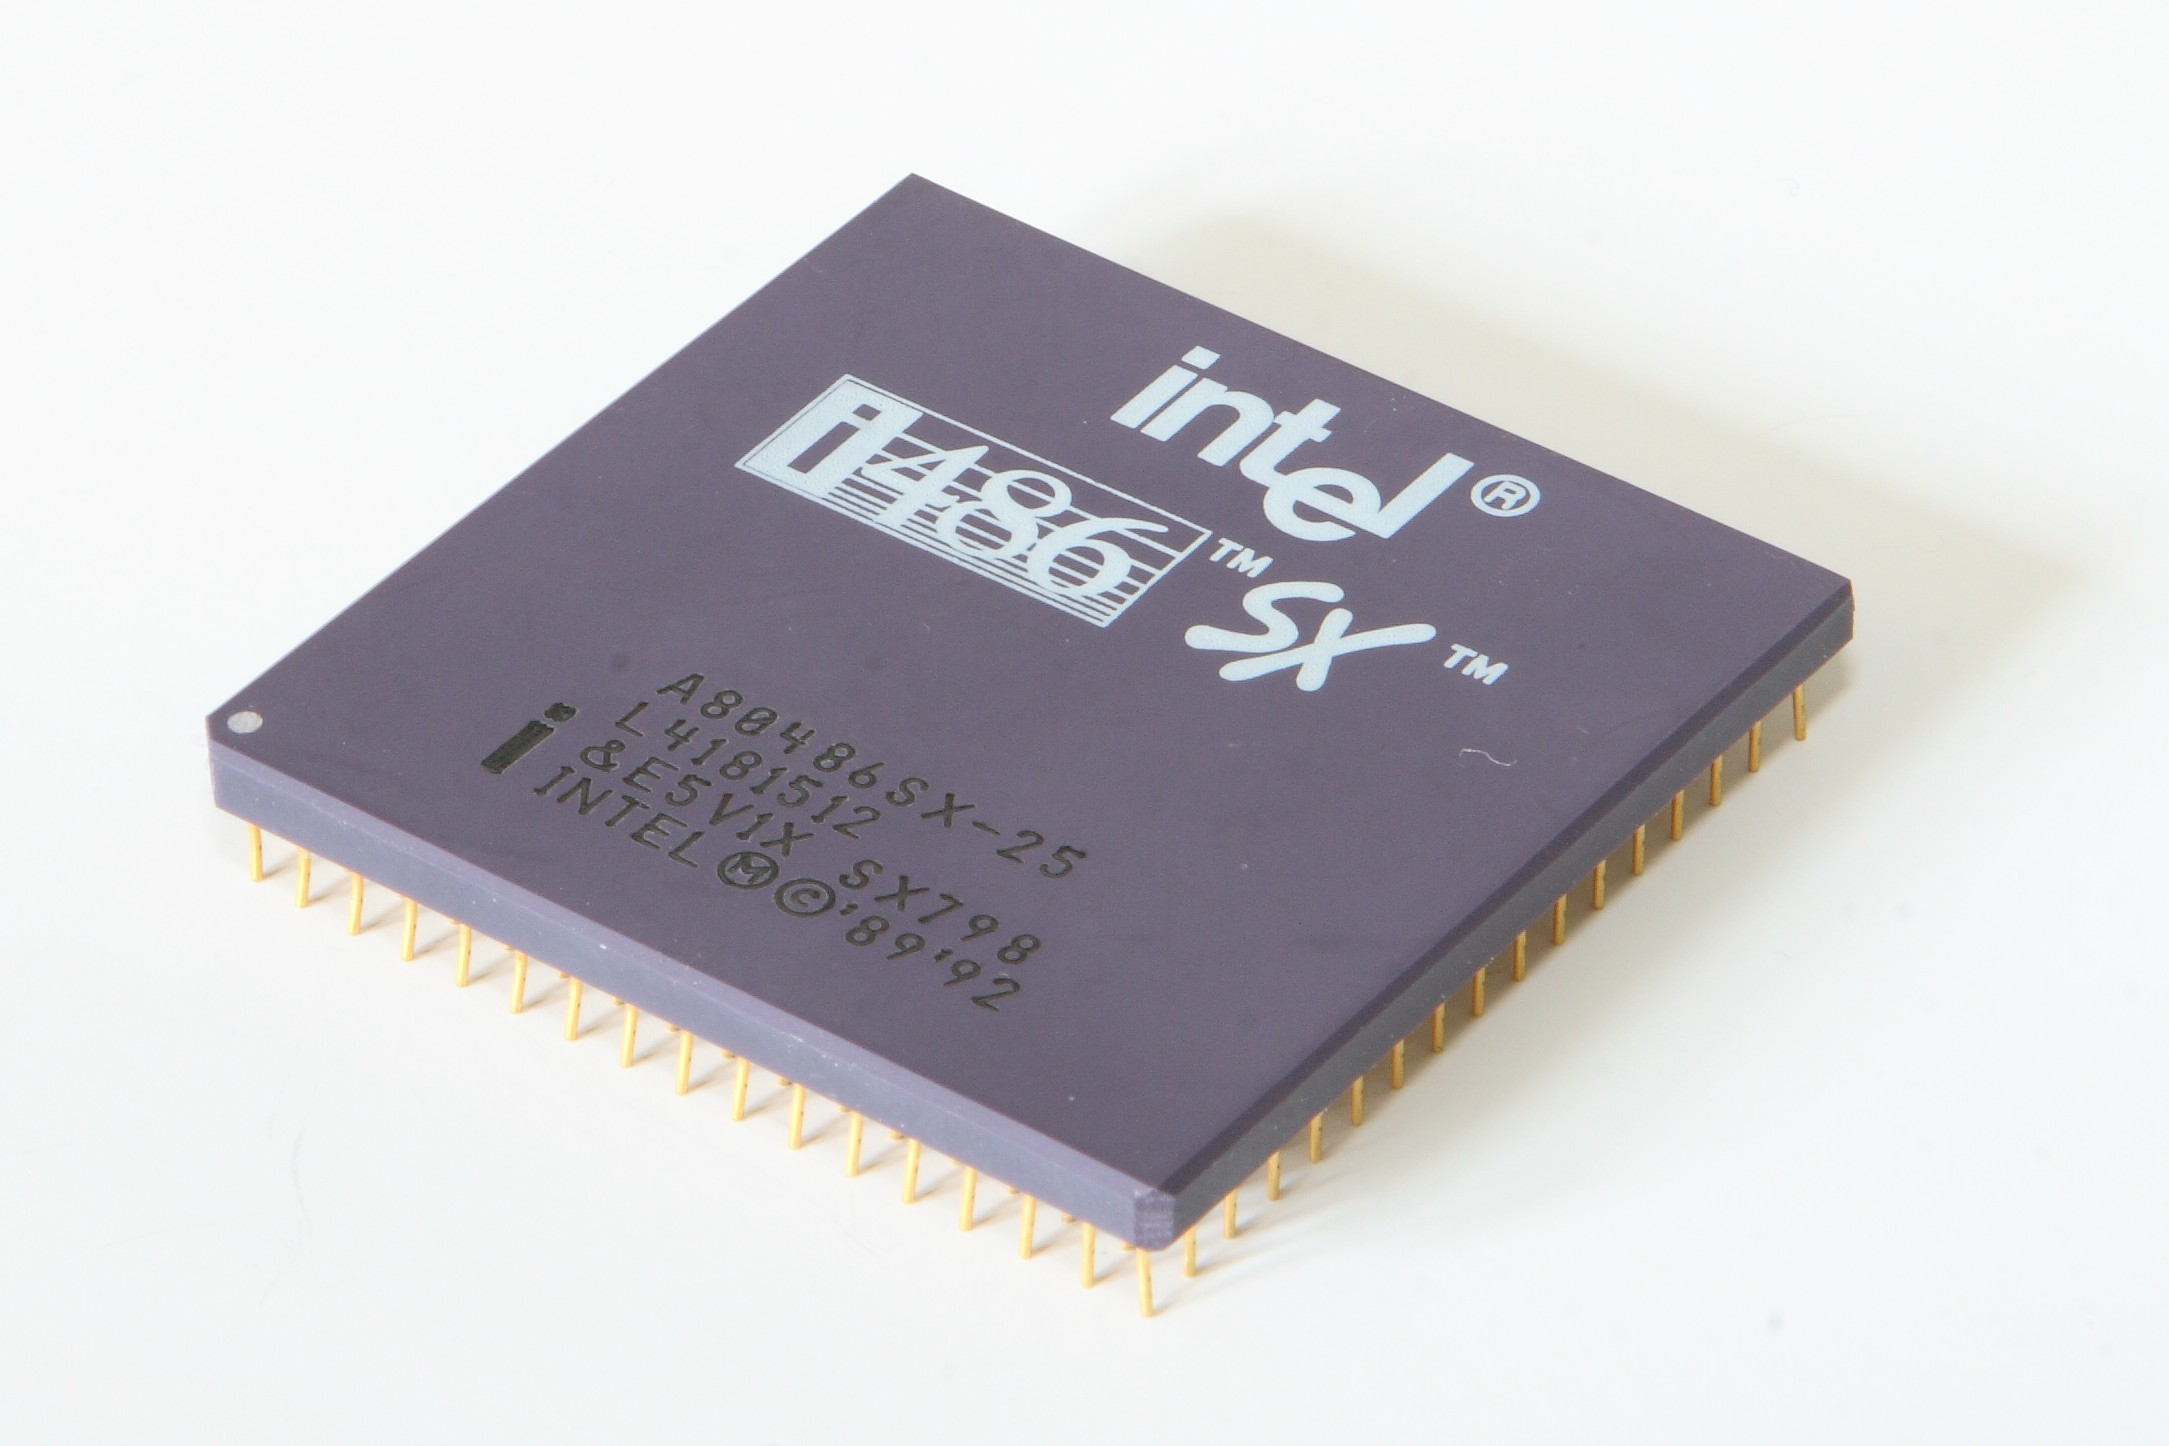
\includegraphics[width=4.5cm]{intel486.jpg}
\end{center}
\end{itemize}
\end{frame}

% ------------------------------------------------------------------------------

\subsection{Aufbau}
\begin{frame}[fragile]
\frametitle{Aufbau}
\begin{Verbatim}[frame=single]
<offset> <opcode> [<arg1>, <arg2>]
\end{Verbatim}
\begin{itemize}
\item {\tt offset} $\rightarrow$ aktuelle Bytezahl, Sprungmarker
\item {\tt opcode, args} $\rightarrow$ Befehl und Argumente
\end{itemize}

\pause
\begin{Verbatim}[frame=single]
0 iinc 0, 1
\end{Verbatim}
\begin{itemize}
\item Befehl {\tt iinc}: Inkrementieren
\item Prefix {\tt i}: $\rightarrow$ integer
\item Argument 1 ({\tt 0}): oberstes Stackelement
\item Argument 2 ({\tt 1}): um 1 erhöhen
\end{itemize}
\end{frame}

% ------------------------------------------------------------------------------

\begin{frame}[fragile]
\frametitle{Aufbau}
\begin{itemize}
\item Prefixe/Suffixe: Datentypen

{\tt {\btt i}  integer, {\btt l} long, {\btt s} short, {\btt b} byte, {\btt c} character\\
{\btt f} float, {\btt d} double, {\btt z} boolean, {\btt a} reference}

\begin{Verbatim}[frame=single]
0 fcmpl
\end{Verbatim}
\pause

\item Suffixe (speziell): {\tt const, load, store} + {\tt \_n}

\begin{Verbatim}[frame=single]
0 iconst_0    // 03                    push int 0 to stack
0 iconst_m1   // 02                   push int -1 to stack
1 sipush 999  // 11 03 E7     push signed int 999 to stack
\end{Verbatim}
\end{itemize}
\end{frame}

% ------------------------------------------------------------------------------

\begin{frame}[fragile]
\frametitle{Aufbau}
\begin{itemize}
\item An Bytegrenzen ausgerichtet
\item JVM-Stack Slotgröße: 4 byte
\begin{itemize}
\item {\tt integer, float, byte, short}: 4 byte/1 Slot
\item {\tt long, double}: 8 byte/2 Slots
\end{itemize}
\end{itemize}
\end{frame}

% ------------------------------------------------------------------------------

\subsection{Instruktionsgruppen}
\begin{frame}{Instruktionsgruppen}
\begin{itemize}
\item Laden/Speichern \hfill {\tt aload\_0, istore}\;\;\;\pause
\item Arithmetische/logische Operationen \hfill {\tt ladd, fcmpl}\;\;\;\pause
\item Typkonversion \hfill {\tt i2b, d2i}\;\;\;\pause
\item Objekterzeugung und -manipulierung \hfill {\tt new, putfield}\;\;\;\pause
\item Operandenstapelmanagement \hfill {\tt swap, dup2}\;\;\;\pause
\item Kontrollübertragung \hfill {\tt ifeq, goto}\;\;\;\pause
\item Methodenausführung \hfill {\tt invokespecial, areturn}\;\;\;
\end{itemize}
\end{frame}

% ------------------------------------------------------------------------------

\section{Beispiel}

\begin{frame}<beamer>{Inhalt}
\tableofcontents[currentsection,currentsubsection]
\end{frame}

\begin{frame}{Bytecode-Ausschnitt}
\tt{\$ javac Example.java}\pause

{\btt\$ javap -c -s -v -l Example}
\end{frame}

% ------------------------------------------------------------------------------

\begin{frame}[fragile,plain]
\frametitle{Bytecode-Ausschnitt}
\begin{lstlisting}[language=Java]
Constant pool:
  #1= Methodref  #5.#15  //java/lang/Object."<init>":()V
  #2= Fieldref   #16.#17 //java/lang/System.out:Ljava/io/PrintStream;
  #3= Methodref  #18.#19 //java/io/PrintStream.println:(I)V

class example.Example {

  example.Example();
     0: aload_0       
     1: invokespecial #1
     4: return    

  public static void main(java.lang.String[]);
     0: iconst_0      
     1: istore_1      
     2: iload_1       
     3: iconst_5      
     4: if_icmpge     20
     7: getstatic     #2
    10: iload_1       
    11: invokevirtual #3
    14: iinc          1, 1
    17: goto          2
    20: return        
}
\end{lstlisting}
\end{frame}

% ------------------------------------------------------------------------------

\begin{frame}[fragile]
\frametitle{Beispielprogramm}
\begin{lstlisting}[language=Java]
class Example {
  
  public static void main(String[] args) {
    for(int i = 0; i < 5; i++) {
      System.out.println(i);
    }
  }

}
\end{lstlisting}
\end{frame}

% ------------------------------------------------------------------------------

\begin{frame}[fragile,plain]
\frametitle{Classfile Teil 1}
\begin{lstlisting}[language=Java,basicstyle=\ttfamily\tiny]
Classfile /data/Repositories/FUBerlin/Semester/ss13/ss13-com/Vortrag/example/Example.class
  Last modified 17.04.2013; size 446 bytes
  MD5 checksum 1f4fd95d93cfdb73b348333b97ca87d2
  Compiled from "Example.java"
class example.Example
  SourceFile: "Example.java"
  minor version: 0
  major version: 51
  flags: ACC_SUPER
Constant pool:
   #1 = Methodref          #5.#15         //  java/lang/Object."<init>":()V
   #2 = Fieldref           #16.#17        //  java/lang/System.out:Ljava/io/PrintStream;
   #3 = Methodref          #18.#19        //  java/io/PrintStream.println:(I)V
   #4 = Class              #20            //  example/Example
   #5 = Class              #21            //  java/lang/Object
   #6 = Utf8               <init>
   #7 = Utf8               ()V
   #8 = Utf8               Code
   #9 = Utf8               LineNumberTable
  #10 = Utf8               main
  #11 = Utf8               ([Ljava/lang/String;)V
  #12 = Utf8               StackMapTable
  #13 = Utf8               SourceFile
  #14 = Utf8               Example.java
  #15 = NameAndType        #6:#7          //  "<init>":()V
  #16 = Class              #22            //  java/lang/System
  #17 = NameAndType        #23:#24        //  out:Ljava/io/PrintStream;
  #18 = Class              #25            //  java/io/PrintStream
  #19 = NameAndType        #26:#27        //  println:(I)V
  #20 = Utf8               example/Example
  #21 = Utf8               java/lang/Object
  #22 = Utf8               java/lang/System
  #23 = Utf8               out
  #24 = Utf8               Ljava/io/PrintStream;
  #25 = Utf8               java/io/PrintStream
  #26 = Utf8               println
  #27 = Utf8               (I)V
{
  example.Example();
    Signature: ()V
    flags: 
    LineNumberTable:
      line 3: 0
\end{lstlisting}
\end{frame}

\begin{frame}[fragile,plain]
\frametitle{Classfile Teil 2}
\begin{lstlisting}[language=Java,basicstyle=\ttfamily\tiny,firstnumber=44]
    Code:
      stack=1, locals=1, args_size=1
         0: aload_0       
         1: invokespecial #1                  // Method java/lang/Object."<init>":()V
         4: return        
      LineNumberTable:
        line 3: 0

  public static void main(java.lang.String[]);
    Signature: ([Ljava/lang/String;)V
    flags: ACC_PUBLIC, ACC_STATIC
    LineNumberTable:
      line 6: 0
      line 7: 7
      line 6: 14
      line 9: 20
    Code:
      stack=2, locals=2, args_size=1
         0: iconst_0      
         1: istore_1      
         2: iload_1       
         3: iconst_5      
         4: if_icmpge     20
         7: getstatic     #2                  // Field java/lang/System.out:Ljava/io/PrintStream;
        10: iload_1       
        11: invokevirtual #3                  // Method java/io/PrintStream.println:(I)V
        14: iinc          1, 1
        17: goto          2
        20: return        
      LineNumberTable:
        line 6: 0
        line 7: 7
        line 6: 14
        line 9: 20
      StackMapTable: number_of_entries = 2
           frame_type = 252 /* append */
             offset_delta = 2
        locals = [ int ]
           frame_type = 250 /* chop */
          offset_delta = 17

}
\end{lstlisting}
\end{frame}

% ------------------------------------------------------------------------------

\begin{frame}{Quellen}
\begin{itemize}
\item The Java Virtual Machine Specification, Java SE 7 Edition\\
\url{http://docs.oracle.com/javase/specs/jvms/se7/html/}\\
insbesondere Kapitel 6: Java Virtual Machine Instruction Set
\item Java Class File Disassembler Documentation\\
\url{http://docs.oracle.com/javase/7/docs/technotes/tools/windows/javap.html}
\item \url{http://en.wikipedia.org/wiki/Java_bytecode}
\item \url{http://www.javaworld.com/jw-09-1996/jw-09-bytecodes.html}
\end{itemize}
\end{frame}

\end{document}
